\documentclass[10pt,letterpaper]{article}
\usepackage{mathpazo}
\usepackage[scaled]{helvet}
\usepackage[T1]{fontenc}
\usepackage{hyperref}
\usepackage{color,soul}
\usepackage{graphicx}
\usepackage[justification=centering,singlelinecheck=false]{caption}
%\usepackage{setspace}
\usepackage[margin=0.75in,includehead,includefoot]{geometry}
\usepackage[table,dvipsnames]{xcolor}
\usepackage{amssymb}
\usepackage{amsmath}
\usepackage{fancyhdr}
\usepackage{array}
\usepackage{gensymb}
\usepackage{lastpage}
\usepackage{textcomp}
\usepackage{booktabs}
\usepackage{pdfpages}
\usepackage{tabto}
\usepackage{multicol}
\usepackage{tabularx}
\usepackage{framed}
\usepackage{chngcntr}
\usepackage{tocloft}
\usepackage[font={sf,normalsize},labelfont={sf,bf}]{caption}
\usepackage{float}
\usepackage{tikz}
\usepackage{listings}
\lstset{basicstyle=\small\ttfamily,breaklines=true}
\usepackage{forest}
\usepackage{verbatim}
\usepackage{longtable}
\usepackage{tabu}
\usepackage{afterpage}
\usepackage{paralist}
\usepackage{indentfirst}

\newenvironment{Figure}
{\par\medskip\noindent\minipage{\linewidth}}
{\endminipage\par\medskip}

%% no indentation
%\setlength{\parindent}{0pt}

%%header and footer
\fancyhf{}
\renewcommand{\footrulewidth}{0pt}
\renewcommand{\headrulewidth}{0pt}
\rhead{\nouppercase{\leftmark}}
\lhead{\sf \textbf{Project 1}  |  Structure Learning}
\rfoot{\sf \textbf{0\thepage} OF \textbf{0\pageref*{LastPage}}}
\rhead{\sf \textbf{AA 228} | Decision Making Under Uncertainty}
\pagestyle{fancy}

%% DOCUMENT START --------------------------------------------------

\begin{document}
		
	\captionsetup[figure]{labelformat=simple, labelsep=quad, labelfont={sf, bf}}
	\captionsetup[table]{labelformat=simple, labelsep=quad, labelfont={sf, bf}}
	
	\section*{\sf \textbf{Bayesian Structure Learning}}
	\vspace*{-0.1 in}
	{\noindent \sf \large R. B. Alexander}
	
	\vspace*{0.2 in}
	
	\noindent \textbf{Bayesian structure learning is a combined structure learning and parameter learning task that involves learning a Bayesian network (or graph) $\mathbf{G}$ from a dataset $\mathbf D$. The dataset contains $\mathbf n$ discrete random variables $\mathbf X_{1:n}$. Each of the variables has $\mathbf r_i$ possible instantiations and for a given graph $\mathbf G$, each of the variables has $\mathbf q_i$ possible instantiations of its parents $\boldsymbol \pi_{ij}$. The number of times $\mathbf X_i = \mathbf k$ given $\boldsymbol\pi_{ij}$ occurs in the dataset is $\mathbf m_{ijk}$ and the associated probability of $\mathbf X_i = \mathbf k$ given $\boldsymbol\pi_{ij}$ is $\mathbf P(\mathbf X_i = \mathbf{k} \mid \boldsymbol\pi_{ij}) = \boldsymbol\theta_{ijk}$. Using the Bayesian score function, we can estimate the likelihood of a graph structure given the dataset. Once we have computed the Bayesian score, we must search the space of all Bayesian networks $\mathbf \mathcal{G}$ to find the graph that maximizes the Bayesian score and is thus, the most probable graph.}
					
	\subsection*{\sf \textbf{Bayesian-Dirichlet Score Function}}
	
	For this project, the Bayesian-Dirichlet scoring function was used, which assumes a Dirichlet prior over the Bayesian network parameters ($P(\boldsymbol\theta) \sim \textnormal{Dir}(\boldsymbol\theta\mid\boldsymbol\alpha)$). The Bayesian-Dirichlet scoring function can be shown to take the following form, where $\Gamma$ is the gamma function, $\Gamma(n) = (n-1)!$.
	
	$$ \ln P(G \mid D) = \ln P(G) + \sum_{i=1}^n\sum_{j=1}^{q_i} \left[ \ln \left( \frac{\Gamma(\alpha_{ij0})}{\Gamma(\alpha_{ij0} + m_{ij0})} \right) + \sum_{k=1}^{r_i} \ln \left( \frac{\Gamma(\alpha_{ijk} + m_{ijk})}{\Gamma(\alpha_{ijk})} \right) \right]$$
	
	$$ \alpha_{ij0} = \sum_{k=1}^{r_i} \alpha_{ijk} \qquad \qquad m_{ij0} = \sum_{k=1}^{r_i} m_{ijk} $$

	Since we have no information about which graph structures are more or less probable, we use a uniform graph prior, $P(G) = 1$. Under weak assumptions, we can assume a uniform Dirichlet prior over the Bayesian network parameters where $\alpha_{ijk} = \alpha$. Here, we set $\alpha = 1$, which gives the K2 scoring function:
	
	$$ \ln P(G \mid D) = \sum_{i=1}^n\sum_{j=1}^{q_i} \left[ \ln \Gamma(r_i) - \ln \Gamma(r_i + m_{ij0}) + \sum_{k=1}^{r_i} \ln \Gamma(1 + m_{ijk})  \right]$$

%	\begin{compactenum}
%		\item \textbf{2 laws of conservation of mass} for $N$ \& $O$
%	\end{compactenum}

	\subsection*{\sf \textbf{Graph Search Algorithms}}
	
	The space of directed acyclic graphs is superexponential with the number of nodes, so an efficient search strategy is critical in finding an optimal Bayesian network. Several algorithms for graph search exist and two relevant classes of these algorithms are directed graph search algorithms and partially-directed graph search algorithms. Two prominent algorithms for directed graph search are K2 search, which greedily adds parents to a node until no higher-scoring graphs are found, and local search, which starts from a graph structure and moves to the highest-scoring graph in its neighborhood (defined by elementary graph operations). Algorithms for partially-directed graph search search the space of Markov equivalence classes, which is smaller than the space of directed graphs. Some algorithms exploit the \textit{score equivalence} of the scoring function to minimally search the space of partially-directed graphs, yielding robust searches.
	
	In our implementation, we used K2 search and added randomized starts to generate several most-probable graphs that could 
		
	\newpage
	
\begin{multicols}{2}
	\begin{Figure} %[t]
		\centering
		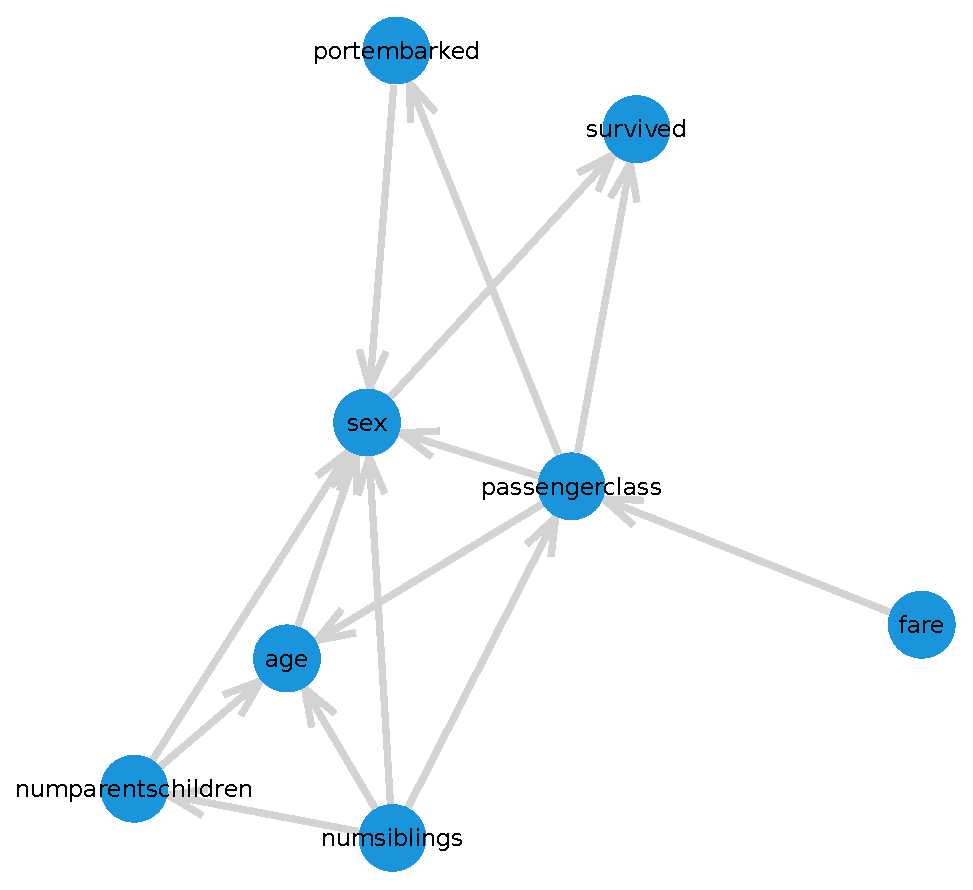
\includegraphics[height=0.32\textheight]{figs/small-K2-1000}
		\setlength{\belowcaptionskip}{-10pt}
		\captionof{figure}{\sf Bayesian network learned from the \texttt{small} dataset (8 variables) using a K2 search of the space of directed acyclic graphs with 1000 randomized starts. ($\ln P(G\mid D) \approx -3795 $)}
		\label{fig:small_graph}
	\end{Figure}

	\begin{Figure} %[t]
		\centering
		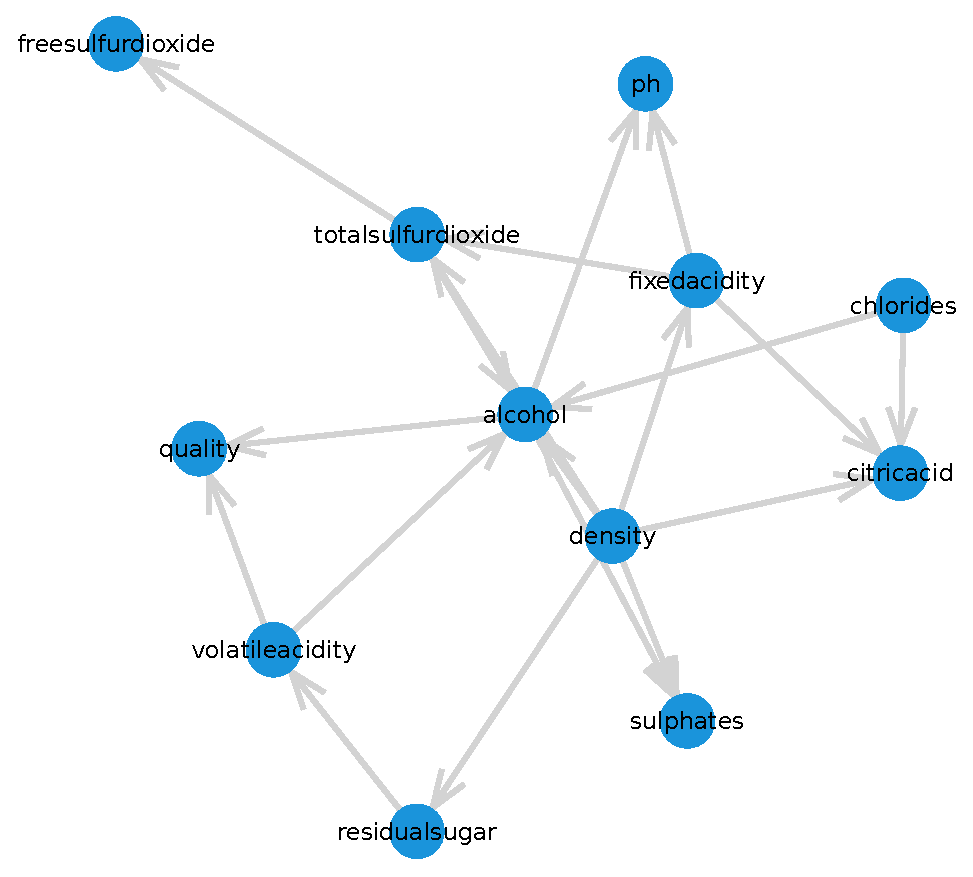
\includegraphics[height=0.32\textheight]{figs/medium-K2-100}
		\setlength{\belowcaptionskip}{-10pt}
		\captionof{figure}{Bayesian network learned from the \texttt{medium} dataset (12 variables) using a K2 search of the space of directed acyclic graphs with 100 randomized starts. ($\ln P(G\mid D) \approx -41961 $)}
		\label{fig:medium_graph}
	\end{Figure}
\end{multicols}	

	\subsubsection*{\sf \textbf{K2 Search}}
	
	\subsubsection*{\sf \textbf{K2 Search with Randomized Start}}
	
	Seeded a random number generator for reproducibility.
	
	Did a K2 search algorithm that iterated over random permutations of variable orderings. Limited the maximum number of parents to 8. Did not do efficient caching or efficient recomputation of the $m_{ijk}$ counts, so the runtimes were long.
	
	describe the strategy you used for your search (e.g. K2) and what modifications (if any) you made to the algorithm. Include any drawbacks that your modifications may have introduced.
	
	provide the timing of how long it took to generate each graph 

	\begin{figure*}[b!]
		\centering
		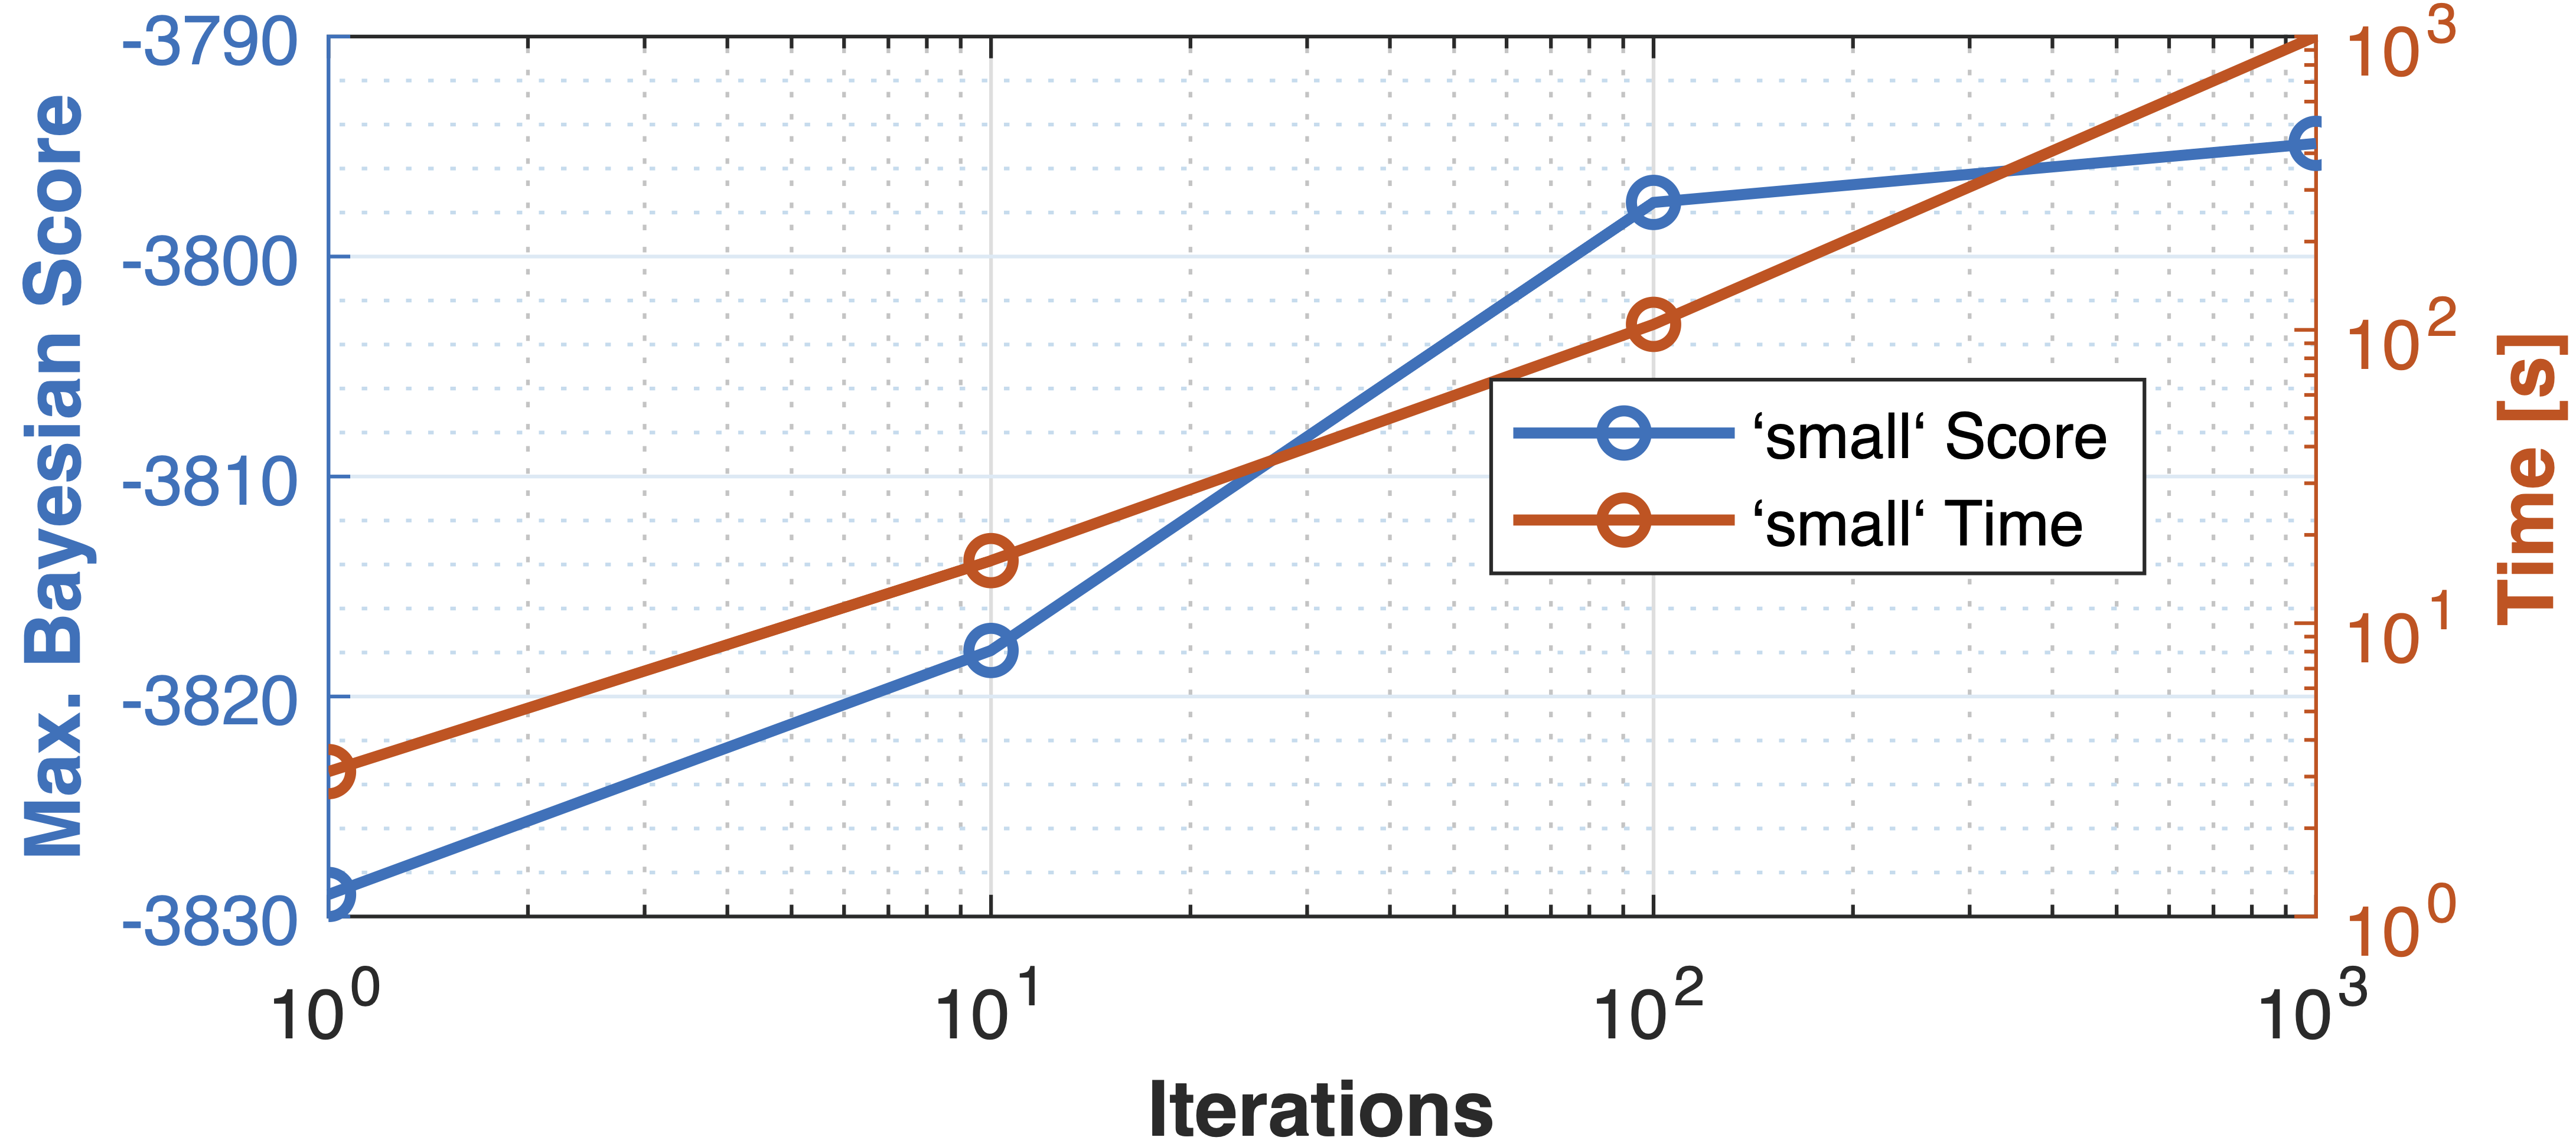
\includegraphics[width=0.4\linewidth]{figs/small-score-time.png}
		\hspace*{0.05\linewidth}
		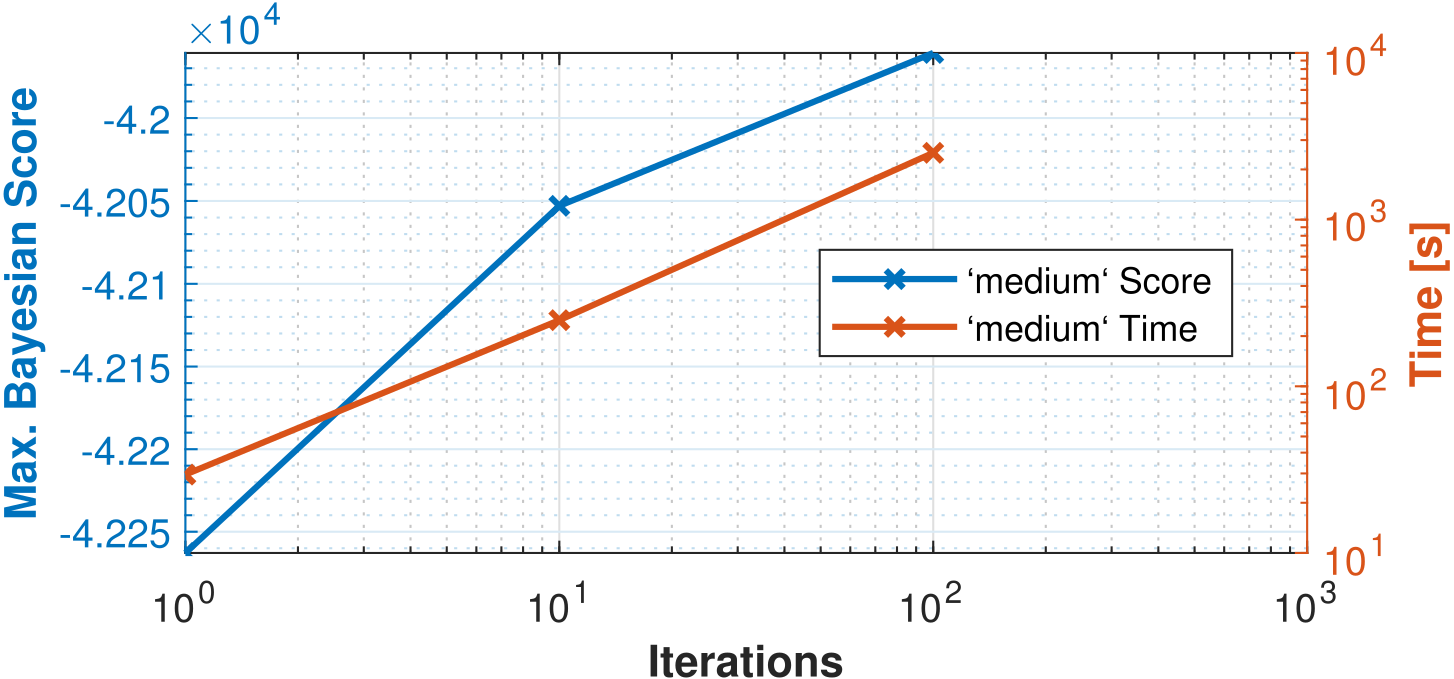
\includegraphics[width=0.4\linewidth]{figs/medium-score-time.png}
		\setlength{\belowcaptionskip}{-10pt}
		\captionof{figure}{Bayesian score improvement using K2 search iterated over randomly-permuted variable orderings.}
		\label{fig:time_score_graph}
	\end{figure*}


	\begin{figure*}[h!] %[t]
		\centering
		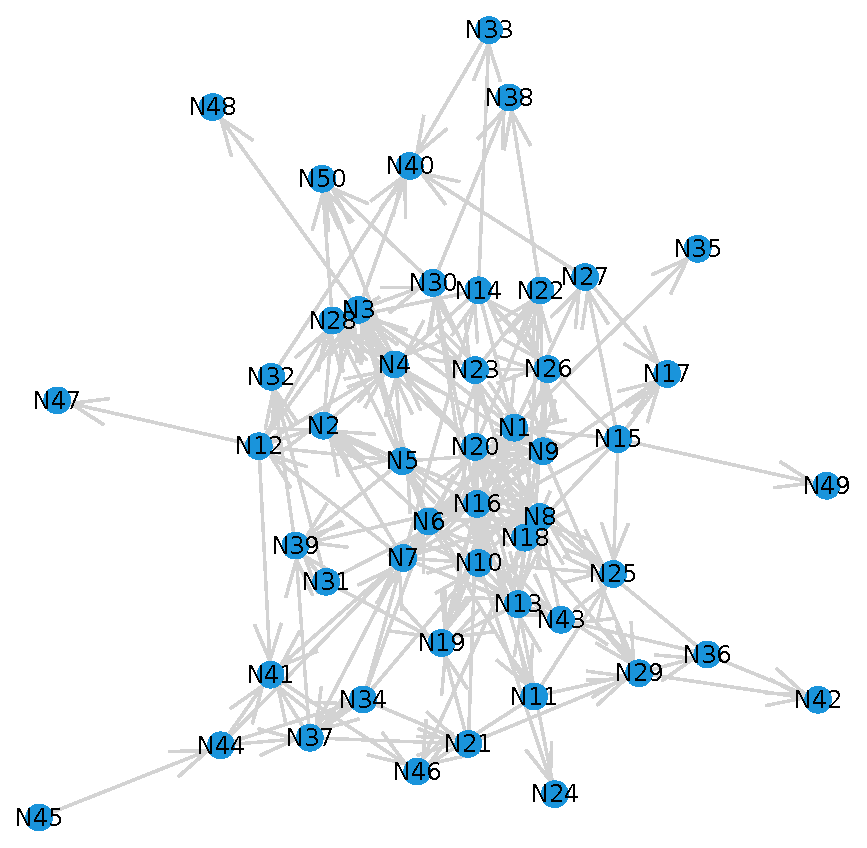
\includegraphics[width=0.9\linewidth]{figs/large-K2-1}
		\setlength{\belowcaptionskip}{-10pt}
		\caption{Bayesian network learned from the \texttt{large} dataset (50 variables) using a K2 search of the space of directed acyclic graphs with 1 randomized start. ($\ln P(G\mid D) \approx - 427612$)}
		\label{fig:large_graph}
	\end{figure*}

				
	
	
	
\end{document}